\chapter{Evaluation}
\label{eval}

\section{Introduction}
In this chapter the two implemented techniques will be evaluated under three read world workloads. In order to show the effect of each configuration parameter, multiple experiments have been designed and deployed. Table~\ref{des:tab:config} defines the configuration space. First, characteristics of workload will be discussed in Section~\ref{eval:workload}. Thereafter, there is separate section for each experiment. Finally, Section~\ref{eval:conc} concludes this chapter.

\section{Workload Characteristic}
\label{eval:workload}

DEBS 2014~\cite{debs2014} has been chosen as a real world workload to test the implementation. Each workload contains data from a random location of the original workload and replayed to feed Spark cluster. All experiments were run for one hour. Figure~\ref{eval:fig:workload} shows distribution of messages in three workloads which have been captured from Spark UI.
\begin{figure}
    \centering
      \begin{subfigure}[h]{\linewidth}
        \centering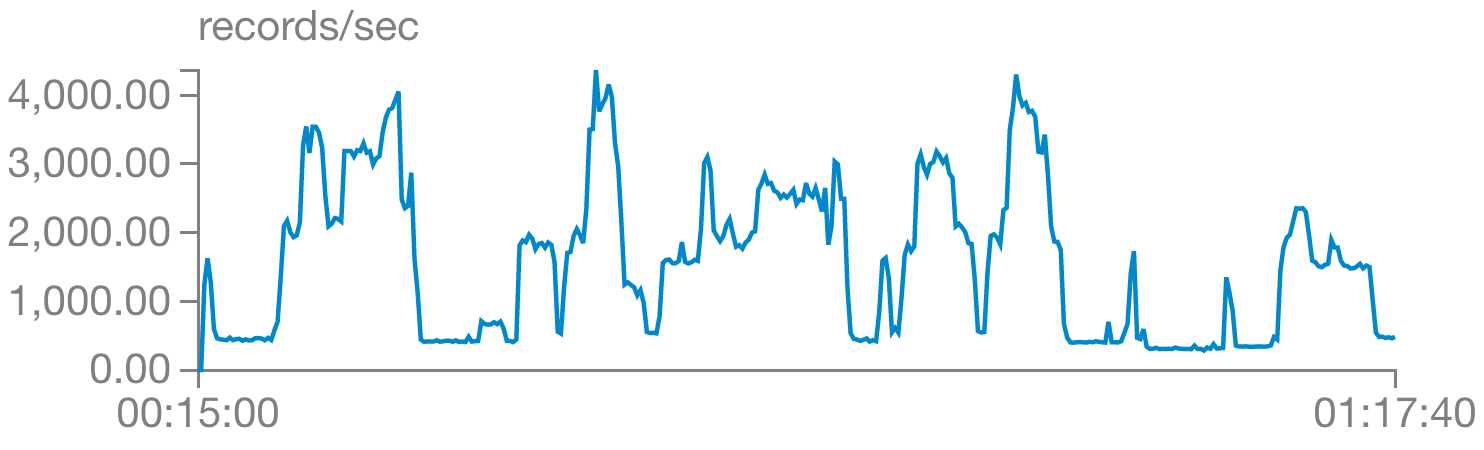
\includegraphics[scale=0.6]{workload1.png}
        \caption{Workload 1}
    \end{subfigure}
    \begin{subfigure}[h]{\linewidth}
        \centering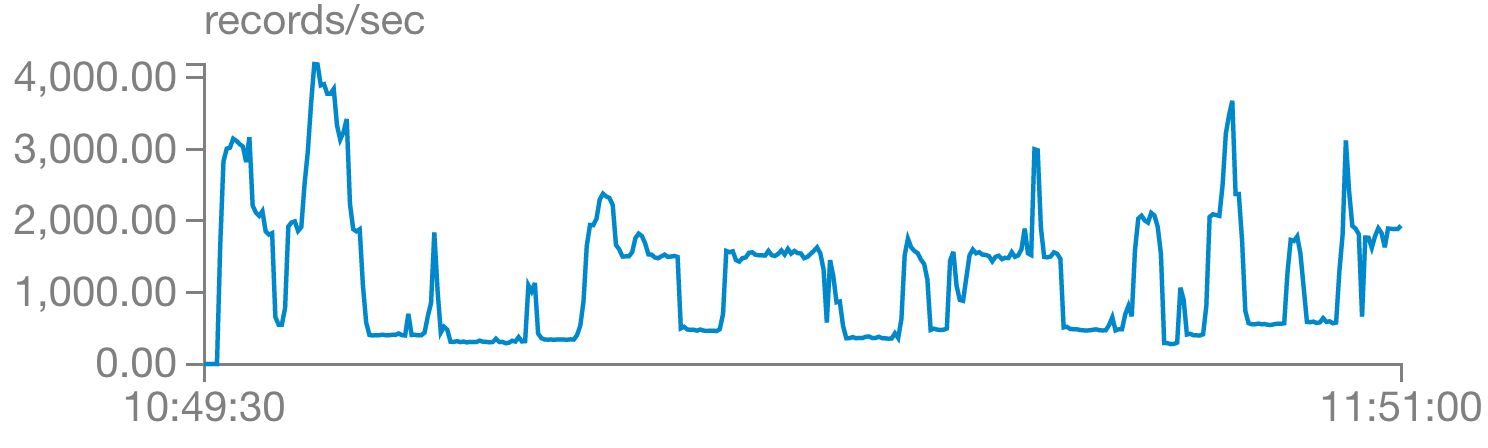
\includegraphics[scale=0.6]{workload2.png}
        \caption{Workload 2}
    \end{subfigure}
    \caption{Three Workloads of DEBS 2014}
    \label{eval:fig:workload}
\end{figure}

The workload involves sensors that measure energy consumption of devices. Each device is connected to one household which in turn is located in one house. This creates a hierarchy from house as parent of households and household as parent of devices. The workload asks to predict energy consumption per device, per household, and per house  for next window of time. The prediction runs over a sliding window of historical measurements which contains $n$ elements. Assuming $window$ variable contains $n$ elements of the history, Equation~\ref{eval:l:pred} defines how the predicted value is calculated.
\begin{equation}
\text{predicted value} = \frac{\text{average(window)} + \text{median(window)}}{2}
\label{eval:l:pred}
\end{equation}

In all experiments \emph{batch size} is set to 10 seconds. The cluster uses 24 executors with minimum of 4 executors that should be respected by Auto-Scaler. All experiments start with minimum number of executors -- 4 in this case -- and run for \emph{one} hour. In case any training is required to run the experiment, training data set is separated from the original workload dataset.

In order to make each workload CPU intensive enough, window size is changed for each workload. Table~\ref{eval:tab:history} defines the history window size for each workload.
\begin{table*}[h]
    \begin{tabular}{lc}
        \toprule
        \textbf{Workload} & \textbf{Window Size = $n$ }\\
        \midrule
        Workload 1 & 1650\\
        Workload 2 & 1900\\
        \bottomrule
    \end{tabular}
    \centering
    \caption{Workload Window Size}
    \label{eval:tab:history}
\end{table*}

\clearpage
\section{Experiment 1: Executor Strategy}
This experiment has been designed to illustrate the strategy of adding/removing executors when taking Scale-In or Scale-Out actions. Table~\ref{eval:tab:ex1} shows the configuration of this experiment.
\begin{table}[h]
    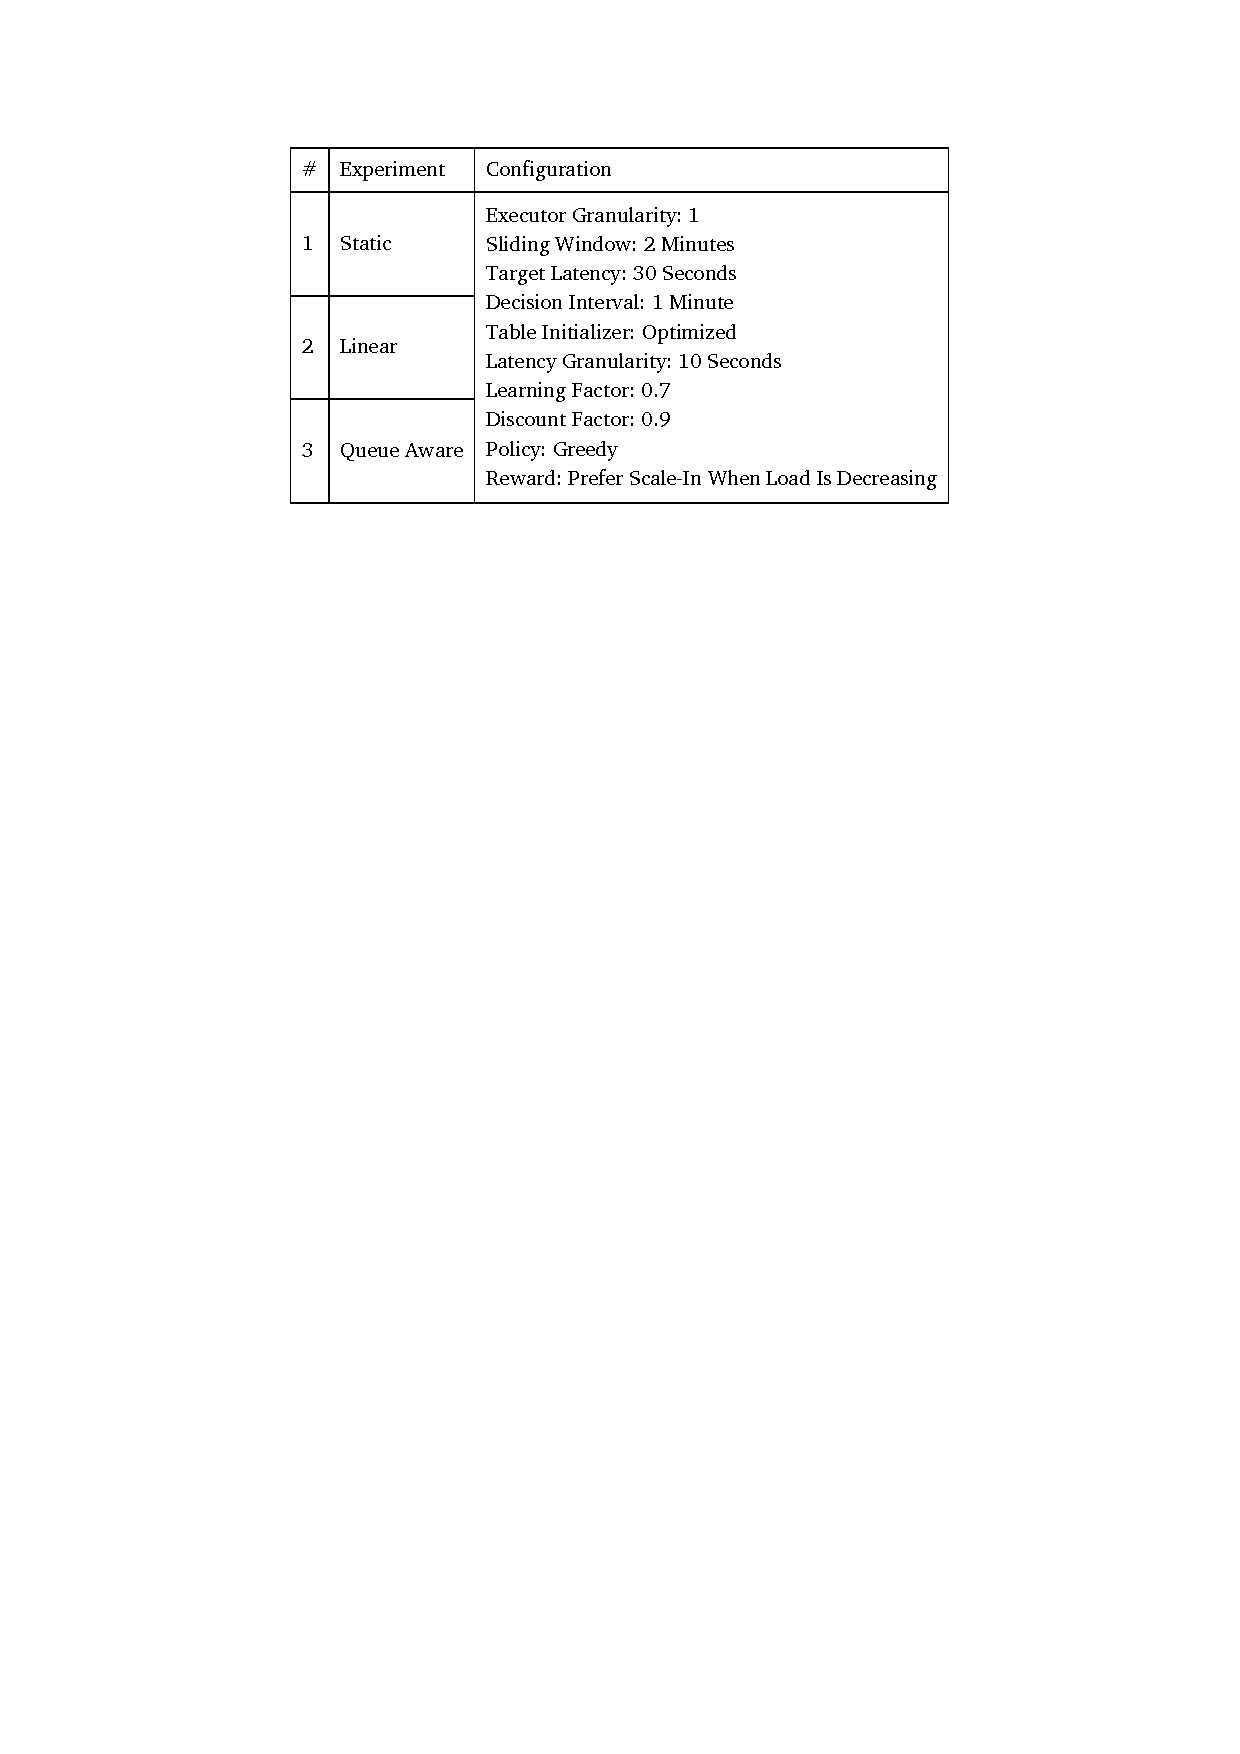
\includegraphics[clip,trim=4.7cm 21.18cm 4.7cm 2.5cm]{tables/ex1.pdf}
    \centering
    \caption{Executor Strategy Configuration Parameters}
    \label{eval:tab:ex1}
\end{table}

Figure~\ref{eval:f:e1:w1:lat},~\ref{eval:f:e1:w1:lat-c} depicts the latency charts. Furthermore, figure~\ref{eval:f:e1:w1:exec},~\ref{eval:f:e1:w1:exec-c} depicts the behavior of strategies regarding number of executors.
\begin{figure}[!htbp]
\centering
\begin{gnuplot}[terminal=epslatex, terminaloptions=color colortext]
set terminal epslatex size 16cm,7.5cm
set key outside center top horizontal
set datafile separator ';'
set xdata time
set timefmt '%H:%M:%S'
set xr ['0:00:00':'1:00:00']
set yr [0:150]
set xtics '00:00:00',600 nomirror
set ytics 0,20 nomirror
set y2r [0:150]
set y2tics 0,20
set samples 50000 
unset mxtics
unset mytics
unset xl
set yl 'Latency (Seconds)'
plot 'ex/e1/w1/latency.csv' using 1:2 w l lc 'red' lw 4 smooth csplines t 'Static',\
'' using 1:3 w l lc 'blue' lw 4 smooth csplines t 'Linear',\
'' using 1:4 w l lc 'black' lw 4 smooth csplines t 'Q-Aware'
\end{gnuplot}
\caption{Executor Strategy -- Workload 1 -- Latency}
\label{eval:f:e1:w1:lat}
\end{figure}
\begin{figure}[!htbp]
	\centering
	\begin{minipage}[h]{\linewidth}
		\centering
		\begin{gnuplot}[terminal=epslatex, terminaloptions=color colortext]
			set terminal epslatex size 16cm,7.5cm
			set key outside center top horizontal
			set datafile separator ';'
			set xr [0.5:3.5]
			set yr [0:150]
			set ytics 0,20 nomirror
			set y2r [0:150]
			set y2tics 0,20
			set boxwidth 0.3 absolute
			set style fill empty
			unset xl
			set yl 'Latency (Seconds)'
			plot 'ex/e1/w1/latency-c.csv' using 1:2:3:4:5:xticlabels(7) with candlesticks lc 'black' lw 4 t 'Min/Max/Percentiles',\
			'' using 1:6:6:6:6 with linespoints pt 5 lc 'black' lw 4 t 'Average' 
		\end{gnuplot}
		\caption{Executor Strategy -- Workload 1 -- Latency -- Min/Max/Percentiles/Average}
		\label{eval:f:e1:w1:lat-c}
	\end{minipage}\hfil
	\begin{minipage}[h]{\linewidth}
		\centering
		\begin{gnuplot}[terminal=epslatex, terminaloptions=color colortext]
			set terminal epslatex size 16cm,7.5cm
			set key outside center top horizontal
			set datafile separator ';'
			set xdata time
			set timefmt '%H:%M:%S'
			set xr ['0:00:00':'1:00:00']
			set yr [2:26]
			set y2r [2:26]
			set ytics 0,4 nomirror
			set xtics '00:00:00',600 nomirror
			set y2tics 0,4
			unset mxtics
			unset mytics
			unset xl
			set yl 'Number of Executors'
			plot 'ex/e1/w1/exec.csv' using 1:2 w l lc 'red' lw 4 t 'Static',\
			'' using 1:3 w l lc 'blue' lw 4 t 'Linear',\
			'' using 1:4 w l lc 'black' lw 4 t 'Q-Aware'
		\end{gnuplot}
		\caption{Executor Strategy -- Workload 1 -- Number of Executors}
		\label{eval:f:e1:w1:exec}
	\end{minipage}\hfil
	\begin{minipage}[h]{\linewidth}
		\centering
		\begin{gnuplot}[terminal=epslatex, terminaloptions=color colortext]
			set terminal epslatex size 16cm,7.5cm
			set key outside center top horizontal
			set datafile separator ';'
			set xr [0.5:3.5]
			set yr [2:26]
			set y2r [2:26]
			set ytics 0,4 nomirror
			set y2tics 0,4 nomirror
			set boxwidth 0.3 absolute
			set style fill empty
			unset xl
			set yl 'Number of Executors'
			plot 'ex/e1/w1/exec-c.csv' using 1:2:3:4:5:xticlabels(7) with candlesticks lc 'black' lw 4 t 'Min/Max/Percentiles',\
			'' using 1:6:6:6:6 with linespoints pt 5 lc 'black' lw 4 t 'Average' 
		\end{gnuplot}
		\caption{Executor Strategy -- Workload 1 -- Number of Executors -- Min/Max/Percentiles/Average}
		\label{eval:f:e1:w1:exec-c}
	\end{minipage}
\end{figure}
\begin{figure}[!htbp]
	\centering
	\begin{minipage}[h]{\linewidth}
		\centering
		\begin{gnuplot}[terminal=epslatex, terminaloptions=color colortext]
			set terminal epslatex size 16cm,7.2cm
			set key outside center top horizontal
			set datafile separator ';'
			set xdata time
			set timefmt '%H:%M:%S'
			set xr ['0:00:00':'1:00:00']
			set yr [0:170]
			set y2r [0:170]
			set xtics '00:00:00',600 nomirror
			set ytics 0,20 nomirror
			set y2tics 0,20
			unset mxtics
			unset mytics
			set samples 50000 
			unset xl
			set yl 'Latency (Seconds)'
			plot 'ex/e1/w2/latency.csv' using 1:2 w l lc 'red' lw 4 smooth csplines t 'Static',\
			'' using 1:3 w l lc 'blue' lw 4 smooth csplines t 'Linear',\
			'' using 1:4 w l lc 'black' lw 4 smooth csplines t 'Q-Aware'
		\end{gnuplot}
		\caption{Executor Strategy -- Workload 2 -- Latency}
		\label{eval:f:e1:w2:lat}
	\end{minipage}\hfil
	\begin{minipage}[h]{\linewidth}
		\centering
		\begin{gnuplot}[terminal=epslatex, terminaloptions=color colortext]
			set terminal epslatex size 16cm,7.2cm
			set key outside center top horizontal
			set datafile separator ';'
			set xr [0.5:3.5]
			set yr [0:170]
			set y2r [0:170]
			set ytics nomirror
			set y2tics 0,20
			set boxwidth 0.3 absolute
			set style fill empty
			unset xl
			set yl 'Latency (Seconds)'
			plot 'ex/e1/w2/latency-c.csv' using 1:2:3:4:5:xticlabels(7) with candlesticks lc 'black' lw 4 t 'Min/Max/Percentiles',\
			'' using 1:6:6:6:6 with linespoints pt 5 lc 'black' lw 4 t 'Average' 
		\end{gnuplot}
		\caption{Executor Strategy -- Workload 2 -- Latency -- Min/Max/Percentiles/Average}
		\label{eval:f:e1:w2:lat-c}
	\end{minipage}\hfil
	\begin{minipage}[h]{\linewidth}
		\centering
		\begin{gnuplot}[terminal=epslatex, terminaloptions=color colortext]
			set terminal epslatex size 16cm,7.2cm
			set key outside center top horizontal
			set datafile separator ';'
			set xdata time
			set timefmt '%H:%M:%S'
			set xr ['0:00:00':'1:00:00']
			set yr [2:26]
			set y2r [2:26]
			set xtics '00:00:00',600 nomirror
			set ytics 0,4 nomirror
			set y2tics 0,4
			unset mxtics
			unset mytics
			unset xl
			set yl 'Number of Executors'
			plot 'ex/e1/w2/exec.csv' using 1:2 w l lc 'red' lw 4 t 'Static',\
			'' using 1:3 w l lc 'blue' lw 4 t 'Linear',\
			'' using 1:4 w l lc 'black' lw 4 t 'Q-Aware'
		\end{gnuplot}
		\caption{Executor Strategy -- Workload 2 -- Number of Executors}
		\label{eval:f:e1:w2:exec}
	\end{minipage}
\end{figure}
\begin{figure}[!htbp]
\centering
\begin{gnuplot}[terminal=epslatex, terminaloptions=color colortext]
set terminal epslatex size 16cm,7.2cm
set key outside center top horizontal
set datafile separator ';'
set xr [0.5:3.5]
set yr [2:26]
set ytics 0,4 nomirror
set y2r [2:26]
set y2tics 0,4
set boxwidth 0.3 absolute
set style fill empty
unset xl
set yl 'Number of Executors'
plot 'ex/e1/w2/exec-c.csv' using 1:2:3:4:5:xticlabels(7) with candlesticks lc 'black' lw 4 t 'Min/Max/Percentiles','' using 1:6:6:6:6 with linespoints pt 5 lc 'black' lw 4 t 'Average' 
\end{gnuplot}
\caption{Executor Strategy -- Workload 2 -- Number of Executors -- Min/Max/Percentiles/Average}
\label{eval:f:e1:w2:exec-c}
\end{figure}
\FloatBarrier
\subsection{Conclusion}

\clearpage
\section{Experiment 2: History Window}
This experiment has been designed to illustrate the effect of history window on quality of decision made by Auto-Scaler. Table~\ref{eval:tab:ex2} shows the configuration of this experiment.
\begin{table}[h]
    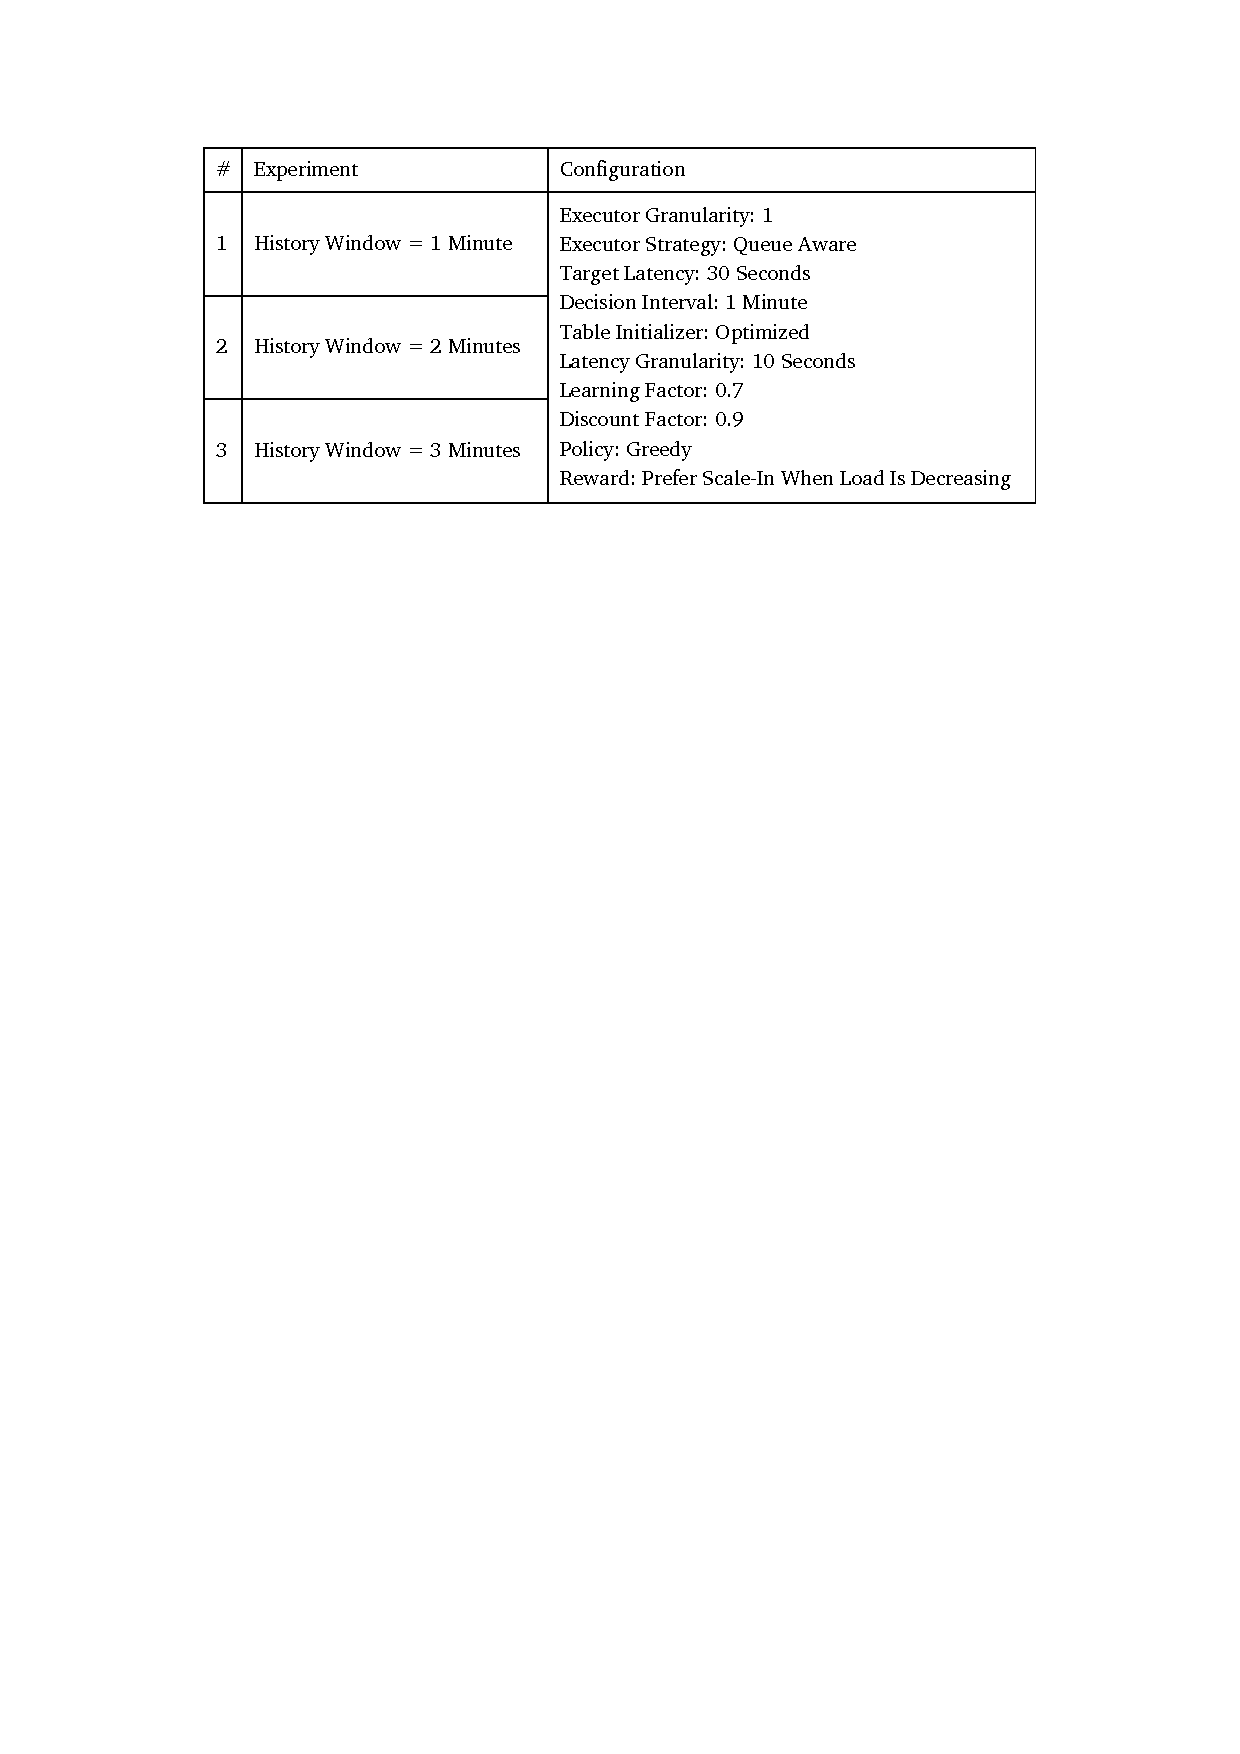
\includegraphics[clip,trim=3.3cm 21.18cm 3.25cm 2.5cm]{tables/ex2.pdf}
    \centering
    \caption{History Window Configuration Parameters}
    \label{eval:tab:ex2}
\end{table}
\begin{figure}[!htbp]
    \centering
    \begin{gnuplot}[terminal=epslatex, terminaloptions=color colortext]
        set terminal epslatex size 16cm,7.5cm
        set key outside center top horizontal
        set datafile separator ';'
        set xdata time
        set timefmt '%H:%M:%S'
        set xr ['0:00:00':'1:00:00']
        set yr [0:110]
        set xtics '00:00:00',600 nomirror
        set ytics 0,20 nomirror
        set y2r [0:110]
        set y2tics 0,20
        set samples 50000 
        unset mxtics
        unset mytics
        unset xl
        set yl 'Latency (Seconds)'
        plot 'ex/e2/w1/latency.csv' using 1:2 w l lc 'red' lw 4 smooth csplines t '1 Min',\
        '' using 1:3 w l lc 'blue' lw 4 smooth csplines t '2 Min',\
        '' using 1:4 w l lc 'black' lw 4 smooth csplines t '3 Min'
    \end{gnuplot}
    \caption{History Window -- Workload 1 -- Latency}
    \label{eval:f:e2:w1:lat}
\end{figure}
\begin{figure}[!htbp]
    \centering
    \begin{minipage}[h]{\linewidth}
        \centering
        \begin{gnuplot}[terminal=epslatex, terminaloptions=color colortext]
            set terminal epslatex size 16cm,7.5cm
            set key outside center top horizontal
            set datafile separator ';'
            set xr [0.5:3.5]
            set yr [0:110]
            set ytics 0,20 nomirror
            set y2r [0:110]
            set y2tics 0,20
            set boxwidth 0.3 absolute
            set style fill empty
            unset xl
            set yl 'Latency (Seconds)'
            plot 'ex/e2/w1/latency-c.csv' using 1:2:3:4:5:xticlabels(7) with candlesticks lc 'black' lw 4 t 'Min/Max/Percentiles',\
            '' using 1:6:6:6:6 with linespoints pt 5 lc 'black' lw 4 t 'Average' 
        \end{gnuplot}
        \caption{History Window -- Workload 1 -- Latency}
        \label{eval:f:e2:w1:lat-c}
    \end{minipage}\hfil
    \begin{minipage}[h]{\linewidth}
        \centering
        \begin{gnuplot}[terminal=epslatex, terminaloptions=color colortext]
            set terminal epslatex size 16cm,7.5cm
            set key outside center top horizontal
            set datafile separator ';'
            set xdata time
            set timefmt '%H:%M:%S'
            set xr ['0:00:00':'1:00:00']
            set yr [2:26]
            set y2r [2:26]
            set ytics 0,4 nomirror
            set xtics '00:00:00',600 nomirror
            set y2tics 0,4
            unset mxtics
            unset mytics
            unset xl
            set yl 'Number of Executors'
            plot 'ex/e2/w1/exec.csv' using 1:2 w l lc 'red' lw 4 t '1 Min',\
            '' using 1:3 w l lc 'blue' lw 4 t '2 Min',\
            '' using 1:4 w l lc 'black' lw 4 t '3 Min'
        \end{gnuplot}
        \caption{History Window -- Workload 1 -- Number of Executors}
        \label{eval:f:e2:w1:exec}
    \end{minipage}\hfil
    \begin{minipage}[h]{\linewidth}
        \centering
        \begin{gnuplot}[terminal=epslatex, terminaloptions=color colortext]
            set terminal epslatex size 16cm,7.5cm
            set key outside center top horizontal
            set datafile separator ';'
            set xr [0.5:3.5]
            set yr [2:26]
            set y2r [2:26]
            set ytics 0,4 nomirror
            set y2tics 0,4 nomirror
            set boxwidth 0.3 absolute
            set style fill empty
            unset xl
            set yl 'Number of Executors'
            plot 'ex/e2/w1/exec-c.csv' using 1:2:3:4:5:xticlabels(7) with candlesticks lc 'black' lw 4 t 'Min/Max/Percentiles',\
            '' using 1:6:6:6:6 with linespoints pt 5 lc 'black' lw 4 t 'Average' 
        \end{gnuplot}
        \caption{History Window -- Workload 1 -- Number of Executors}
        \label{eval:f:e2:w1:exec-c}
    \end{minipage}
\end{figure}
\begin{figure}[!htbp]
    \centering
    \begin{minipage}[h]{\linewidth}
        \centering
        \begin{gnuplot}[terminal=epslatex, terminaloptions=color colortext]
            set terminal epslatex size 16cm,7.2cm
            set key outside center top horizontal
            set datafile separator ';'
            set xdata time
            set timefmt '%H:%M:%S'
            set xr ['0:00:00':'1:00:00']
            set yr [0:130]
            set y2r [0:130]
            set xtics '00:00:00',600 nomirror
            set ytics 0,20 nomirror
            set y2tics 0,20
            unset mxtics
            unset mytics
            set samples 50000 
            unset xl
            set yl 'Latency (Seconds)'
            plot 'ex/e2/w2/latency.csv' using 1:2 w l lc 'red' lw 4 smooth csplines t '1 Min',\
            '' using 1:3 w l lc 'blue' lw 4 smooth csplines t '2 Min',\
            '' using 1:4 w l lc 'black' lw 4 smooth csplines t '3 Min'
        \end{gnuplot}
        \caption{History Window -- Workload 2 -- Latency}
        \label{eval:f:e2:w2:lat}
    \end{minipage}\hfil
    \begin{minipage}[h]{\linewidth}
        \centering
        \begin{gnuplot}[terminal=epslatex, terminaloptions=color colortext]
            set terminal epslatex size 16cm,7.2cm
            set key outside center top horizontal
            set datafile separator ';'
            set xr [0.5:3.5]
            set yr [0:130]
            set y2r [0:130]
            set ytics nomirror
            set y2tics 0,20
            set boxwidth 0.3 absolute
            set style fill empty
            unset xl
            set yl 'Latency (Seconds)'
            plot 'ex/e2/w2/latency-c.csv' using 1:2:3:4:5:xticlabels(7) with candlesticks lc 'black' lw 4 t 'Min/Max/Percentiles',\
            '' using 1:6:6:6:6 with linespoints pt 5 lc 'black' lw 4 t 'Average' 
        \end{gnuplot}
        \caption{History Window -- Workload 2 -- Latency}
        \label{eval:f:e2:w2:lat-c}
    \end{minipage}\hfil
    \begin{minipage}[h]{\linewidth}
        \centering
        \begin{gnuplot}[terminal=epslatex, terminaloptions=color colortext]
            set terminal epslatex size 16cm,7.2cm
            set key outside center top horizontal
            set datafile separator ';'
            set xdata time
            set timefmt '%H:%M:%S'
            set xr ['0:00:00':'1:00:00']
            set yr [2:26]
            set y2r [2:26]
            set xtics '00:00:00',600 nomirror
            set ytics 0,4 nomirror
            set y2tics 0,4
            unset mxtics
            unset mytics
            unset xl
            set yl 'Number of Executors'
            plot 'ex/e2/w2/exec.csv' using 1:2 w l lc 'red' lw 4 t '1 Min',\
            '' using 1:3 w l lc 'blue' lw 4 t '2 Min',\
            '' using 1:4 w l lc 'black' lw 4 t '3 Min'
        \end{gnuplot}
        \caption{History Window -- Workload 2 -- Number of Executors}
        \label{eval:f:e2:w2:exec}
    \end{minipage}
\end{figure}
\begin{figure}[!htbp]
    \centering
    \begin{gnuplot}[terminal=epslatex, terminaloptions=color colortext]
        set terminal epslatex size 16cm,7.2cm
        set key outside center top horizontal
        set datafile separator ';'
        set xr [0.5:3.5]
        set yr [2:26]
        set ytics 0,4 nomirror
        set y2r [2:26]
        set y2tics 0,4
        set boxwidth 0.3 absolute
        set style fill empty
        unset xl
        set yl 'Number of Executors'
        plot 'ex/e2/w2/exec-c.csv' using 1:2:3:4:5:xticlabels(7) with candlesticks lc 'black' lw 4 t 'Min/Max/Percentiles','' using 1:6:6:6:6 with linespoints pt 5 lc 'black' lw 4 t 'Average' 
    \end{gnuplot}
    \caption{History Window -- Workload 2 -- Number of Executors}
    \label{eval:f:e2:w2:exec-c}
\end{figure}
\FloatBarrier
\subsection{Conclusion}

\clearpage
\section{Experiment 3: Decision Interval}